\documentclass[svgnames]{article}     % use "amsart" instead of "article" for AMSLaTeX format
%\geometry{landscape}                 % Activate for rotated page geometry

%\usepackage[parfill]{parskip}        % Activate to begin paragraphs with an empty line rather than an indent

\usepackage{graphicx}                 % Use pdf, png, jpg, or eps§ with pdflatex; use eps in DVI mode

%maths                                % TeX will automatically convert eps --> pdf in pdflatex
\usepackage{amssymb}
\usepackage{amsmath}
\usepackage{esint}
\usepackage{geometry}

\usepackage{pgfplots,mathtools}
\pgfplotsset{compat=newest}

\let\Re\relax
\DeclareMathOperator{\Re}{Re}
\let\Im\relax
\DeclareMathOperator{\Im}{Im}

% Inverting Color of PDF
%\usepackage{xcolor}
%\pagecolor[rgb]{0.19,0.19,0.19}
%\color[rgb]{0.77,0.77,0.77}

%noindent
\setlength\parindent{0pt}

%pgfplots
\usepackage{pgfplots}

%images
\graphicspath{{/Users/devaldeliwala/screenshots/}}                   % Activate to set a image directory

%tikz
\usepackage{pgfplots}
\pgfplotsset{compat=1.15}
\usepackage{comment}
\usetikzlibrary{arrows}
\usepackage[most]{tcolorbox}

%Figures
\usepackage{float}
\usepackage{caption}
\usepackage{lipsum}


\title{Molecular Effusion \& Mean Free Path}
\author{Deval Deliwala}
%\date{}                              % Activate to display a given date or no date

\begin{document}
\maketitle
%\section{}
%\subsection{}
%\tableofcontents                     % Activate to display a table of contents

\vspace{70px}
\begin{center}
  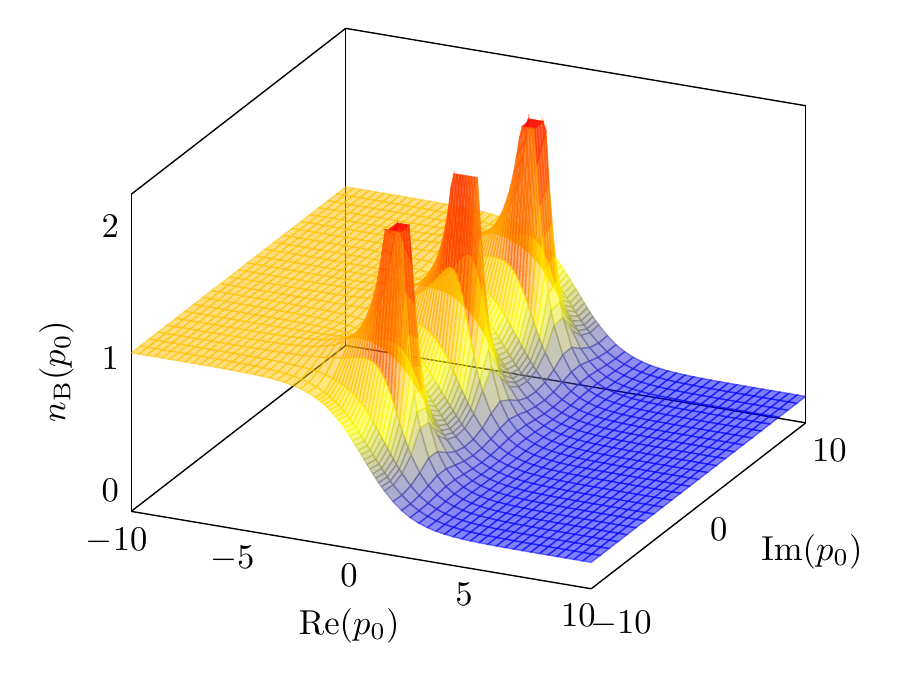
\begin{tikzpicture}[scale = 1.25]
  \begin{axis}[
      xlabel=$\Re(p_0)$,
      ylabel=$\Im(p_0)$,
      zlabel=$n_\text{B}(p_0)$,
      x label style={at={(0.35, 0)}},
      y label style={at={(0.95, 0.15)}},
      shader=flat,
      tickwidth=0pt
    ]

    \def\nB{(e^(2*x) - 2*e^x*cos(deg(y)) + 1)^(-1/2)}

    \addplot3[surf, opacity=0.5, domain=1:10, y domain=-10:10]{\nB};

    \addplot3[surf, opacity=0.5, domain=-10:-2, y domain=-10:10]{\nB};

    \addplot3[surf, opacity=0.5, domain=-2:1, y domain=-10:10, restrict z to domain*=0:2]{\nB};

  \end{axis}
\end{tikzpicture}
\end{center}

\newpage

\tableofcontents

\newpage

\section{Molecular Effusion} 

\textbf{Effusion} is the process by which gas escapes from a small hole. We
begin by first evaluating the flux of particles hitting the inside walls of
a container of gas. 

\subsection{Flux}

Of relevance to this section, the molecular flux, $\Phi$, is defined to be the
\# molecules striking unit area per second. 

\[
  \Phi = \frac{\text{number of molecules}}{\text{area } \times \text{ time}}
\] \vspace{5px}

As derived in the previous chapter, the \# of molecules hitting unit area of
wall in unit time, with speeds between $v$ and $v + dv$ and traveling at angles
between $\theta$ and $\theta + d\theta$ is given by 

\[
v \cos \theta n f(v) \, dv \frac{1}{2}\sin\theta \, d\theta
\] \vspace{5px}

Therefore, the flux of molecules in a gas can be evaluated by integrating over
all $v$ and $\theta$ so that

 \begin{align*}
   \Phi &= \int_{0}^{\infty} \int_{0}^{\pi/2} v\cos\theta n f(v)
   \frac{1}{2}\sin\theta \, d\theta \, dv \\
        &= \frac{n}{2}\int_{0}^{\infty} vf(v) \, dv \int_{0}^{\pi/2}
        \cos\theta\sin\theta \, d\theta
\end{align*}

which yields 

\[
  \boxed{\Phi = \frac{1}{4}n\langle v \rangle}
\] \vspace{5px}

If we define $n$ by rearranging the ideal gas law, 

\[
n = \frac{p}{kT}
\] \vspace{5px}

and using the expression for the average speed of molecules in a gas, 

\[
\langle v \rangle = \sqrt{\frac{8kT}{m}}
\] \vspace{5px}

we can derive a more precise definition for molecular flux: 

\[
  \boxed{ \Phi = \frac{p}{\sqrt{2\pi m kT}}}
\] \vspace{5px}

\subsection{Effusion}

Consider a container of gas with a small hole of area $A$. Gas will leak out of
the hole. The hole is small so that the equilibrium of gas in the container is
not disturbed. The \# of molecules escaping per unit time is just the \# of
molecules hitting the hole area in the closed box per second, so is given by
$\Phi A$. This is the \textbf{effusion rate}. 

\[
  \Phi A = \frac{pA}{\sqrt{2\pi m kT}}
\] \vspace{5px}

Effusion preferentially selects faster molecules. Therefore the speed
distribution of molecules effusing out the hole is not Maxwellian. Faster
molecules inside the box travel more quickly and have a greater probability of
reaching the hole than their slower counterparts. Mathematically, we get an
extra factor of $v$ for the distribution of molecules effusing in some interval
of time: 

\[g(v) \propto v^3e^{-mv^2 / 2k_B T}\] \vspace{5px}


\begin{figure}[H]
  \centering
    \includegraphics[width = 7cm]{screenshot 30.png}
\end{figure}


Maxwellian gas has an average energy of $E_{KE} = \frac{1}{2}m\langle v^2
\rangle = \frac{3}{2}k_B T$. Let's calculate the mean kinetic energy of
molecules effusing out of a small hole. 

\begin{align*}
  \langle E_{KE} \rangle &= \frac{1}{2}m\langle v^2 \rangle \\
                         &= \frac{\frac{1}{2}m \int_{0}^{\infty} v^2 v^3
                         e^{-\frac{1}{2}v^2 / k_B T} \, dv}{\int_{0}^{\infty}
                       v^3 e^{-\frac{1}{2} mv^2 / k_B T} \, dv} \\
                         &= \frac{1}{2}m \left( \frac{2k_B T}{m} \right)
                         \frac{\int_{0}^{\infty} u^2 e^{-u} \,
                         du}{\int_{0}^{\infty} ue^{-u} \, du} 
\end{align*}

where the substitution $u = mv^2 / 2k_B T$ was made. Using the standard
integral, 

\[
  \int_{0}^{\infty} x^n e^{-x} \, dx = n!,
\] \vspace{5px}

we have that 

\[
  \langle E_{KE} \rangle = 2k_B T
\] \vspace{5px}

which is larger by a factor of $\frac{4}{3}$ than the mean kinetic energy of
molecules in the gas.

\subsection{Chapter Summary}

The molecular flux, $\Phi$ is the \# of molecules striking unit area per second
and is given by 

\[
\Phi = \frac{1}{4}n\langle v \rangle
\] \vspace{5px}

This expression, together with the ideal gas law helps us derive an alternative
expression for molecular flux: 

\[
  \Phi = \frac{p}{\sqrt{2\pi m k_B T}}
\] \vspace{5px}

The average kinetic energy of molecules \textit{effusing} out of the container: 

\[
  \langle E_{KE} \rangle = 2k_B T
\] \vspace{5px}

which is $\frac{4}{3}$ larger than the mean kinetic energy of molecules
\textit{in} the gas -- $\frac{3}{2}k_B T$

\newpage
\section{The Mean Free Path \& Collisions}

Processes such as the diffusion of one gas into another would be instantaneous
were it not for the occurrence of \textit{collisions} between molecules.
Collisions are fundamentally quantum mechanical, but in a dilute gas, molecules
spend most of their time between collisions so we can consider them as
classical billiard balls and ignore the details of what \textit{actually
happens} during a collision. All we care about is that after collisions
molecules velocities become essentially randomized. In this section we model
the effect of collisions in a gas and develop concepts of mean collision time,
the collision cross section, and mean free path.

\subsection{The Mean Collision Time}

We aim to calculate the average time molecules spend between collisions. Let's
consider a molecule moving in a gas of other similar molecules. To make things
simple to start with, we suppose that the molecule under consideration is
traveling at speed $v$ and that the other molecules in the gas are stationary.
We also attribute a collision cross-section $\sigma$ to our molecule
\\
In a time $dt$, our molecule sweeps out a volume $\sigma v dt$. If another
molecule happens to lie inside this volume, a collision will occur. With $n$
molecules per unit volume, the probability of a collision in time $dt$ is
therefore $n\sigma v dt$. Let us define $P(t)$ as follows: 

\[
  P(t) = \text{ the probability of a molecule NOT colliding up to time $t$ }
\] \vspace{5px}

Elementary calculus then implies 

\[
P(t + dt) = P(t) + \frac{dP}{dt}dt, 
\] \vspace{5px}

but $P(t+dt)$ is also the probability of a molecule not colliding up to time
$t$ \textit{multiplied} by the probability of not colliding in subsequent time
$dt$, i.e.,

\[
P(t+dt) = P(t)(1-n\sigma v dt)
\] \vspace{5px}

Rearranging gives us 

\[
\frac{1}{P}\frac{dP}{dt} = -n\sigma v
\] \vspace{5px}

Solving yields 

\[
  P(t) = P_0  e^{-n\sigma vt} = e^{-n\sigma vt}
\] \vspace{5px}

Now the probability of surviving without collision up to time $t$ but then
colliding in the next $dt$ is 

\[
  e^{-n\sigma vt} n\sigma v dt
\] \vspace{5px}

We can check this is a solid probability by integrating it: 

\[
  \int_{0}^{\infty}  e^{-n\sigma vt} n\sigma  v \, dt = 1 
\] \vspace{5px}

we can now calculate the \textbf{mean scattering time} $\tau$, which is the
average time elapsed between collisions for a given molecule: 

\begin{align*}
  \tau &= \int_{0}^{\infty} te^{-n\sigma vt} n\sigma v \, dt\\
       &= \frac{1}{n\sigma v} \int_{0}^{\infty} (n\sigma vt) e^{-n\sigma vt} \,
       d(n\sigma vt) \\ 
       &= \frac{1}{n\sigma v}\int_{0}^{\infty} xe^{-x} \, dx
\end{align*}


We find that 

\[
\tau = \frac{1}{n\sigma v}
\] \vspace{5px}

\subsection{The Collision Cross-Section} 

Consider two spherical molecules of radii $a_1$ and $a_2$. 

\begin{figure}[H]
  \centering
    \includegraphics[width = 5cm]{screenshot 31.png}
\end{figure}

A collision will only take place if the center of these other molecules comes
inside a tube of radius $a_1 + a_2$. Thus our first molecule can be considered
to sweep out an imaginary tube space of cross-sectional area $\pi(a_1+a_2)^2$
that defines its ``personal space." The area of this tube is called the
\textbf{collision cross-section} $\sigma$ and is then given by 

\[
\sigma = \pi(a_1 + a_2)^2.
\] \vspace{5px}

If all the molecules are the same (have the same diameter $d$), 

\[
\sigma = \pi d^2
\] \vspace{5px}

\begin{figure}[H]
  \centering
    \includegraphics[width = 10cm]{screenshot 32.png}
\end{figure}

\subsection{The Mean Free Path}

Having derived the mean collision time, it is tempting to derive the
\textbf{mean free path} as 

\[
\lambda = \langle v \rangle \tau = \frac{\langle v \rangle}{n\sigma v}. 
\] \vspace{5px}

But what should we use for $v$?. Our approach to determining the mean collision
timed assumed all other molecules are stationary. The reality is that all
molecules whizz around extremely fast. We should therefore take $v$ as the
average \textit{relative} velocity $\langle v_r \rangle$, where

\[
  \vec{v_r} = \vec{v_1} - \vec{v_2}
\] \vspace{5px}

Therefore, 

\[
\langle v_r ^2 \rangle = \langle v_1 ^2 \rangle + \langle v_2^2 \rangle
- 2\vec{v_1}\cdot \vec{2}
\] \vspace{5px}

which yields 

\[
\langle v^2 \rangle = \langle v_1^2 \rangle + \langle v_2^2 \rangle = 2\langle
v^2 \rangle
\] \vspace{5px}

And since $\langle \vec{v_1} \cdot \vec{v_2} \rangle = 0$ (all molecules are
moving in random directions so $\langle \cos \theta \rangle = 0$. However, the
quantity we want is $\langle v_r \rangle$, not $\langle v_r ^2 \rangle$. If the
probability distribution describing molecular speed is the Maxwellian
Distribution, then the error in writing $\langle v_r \rangle \approx
\sqrt{\langle v_r ^2 \rangle}$ is only around 8\%. So to a reasonable degree of
approximation we can write 

\[
\langle v_r \rangle \approx \sqrt{\langle v_r ^2 \rangle} \approx
\sqrt{2}\langle v \rangle
\] \vspace{5px}

Hence, we obtain an expression for $\lambda$ : 

\[
  \boxed{ \lambda = \frac{1}{\sqrt{2}n\sigma}}
\] \vspace{5px}

While this equation was derived using an approximation, it turns out to be
exact. Substitution of $p = nk_B T$ yields the expression: 

\[
  \lambda = \frac{k_B T}{\sqrt{2}p\sigma}
\] \vspace{5px}


\subsection{Chapter Summary}

The mean scattering time is given by 

\[
\tau = \frac{1}{n\sigma \langle v_r \rangle}, 
\] \vspace{5px}

where the collision cross-section is $\sigma = \pi d^2$, and $\langle v_r
\rangle \approx \sqrt{2}\langle v \rangle$. \\

The mean free path is exactly equal to 

\[
  \lambda = \frac{1}{\sqrt{2}n\sigma} = \frac{k_B T}{\sqrt{2}p\sigma}.
\] \vspace{5px}






\end{document}

